%===================================================================================================
\documentclass[]{elsarticle}
%===================================================================================================

\usepackage{amssymb}
\usepackage{graphicx} % Used for inserting pdf as graphics
\usepackage{subcaption}
%\usepackage{subfig}
\usepackage{float} % Used fo0r 'H' float option in figures
\usepackage[hidelinks]{hyperref} % Used for creating a hyperlink to reference parts
\usepackage{textcomp}
\usepackage{multicol}
\usepackage{tikz}
\usepackage{multirow}
\usepackage{url}
\usepackage{color}
\usepackage{mathtools}
\usepackage[ruled,vlined,linesnumbered]{algorithm2e}

%===================================================================================================

\let\proof\relax 				
\let\endproof\relax 
\usepackage{amsthm}

\theoremstyle{definition}
\newtheorem{definition2}{Definition}

\theoremstyle{definition}
\newtheorem{lemma}{Theorem}
%\newcommand{\keywords}[1]{\par\addvspace\baselineskip}
%\noindent\keywordname\enspace\ignorespaces#1}
\newcommand{\ra}{\rightarrow}
\newcommand{\se}{\text{ }}
\newcommand{\sm}{\text{:}}
\newcommand{\mn}{\text{-}}
\newcommand{\comment}[1]{}

%===================================================================================================
\begin{document}
%===================================================================================================

\begin{frontmatter}

\title{Homogenization of Spiking Neural P Systems}

\author[1]{Ren Tristan A. de la Cruz\corref{cor1}}
\ead{radelacruz@up.edu.ph}
\cortext[cor1]{Corresponding Author}
\author[1]{Francis George C. Cabarle}
\ead{fccabarle@up.edu.ph}
\author[2]{Author Three}
\ead{author3@mail.com}

\address[1]
{
Algorithms and Complexity Lab, 
Department of Computer Science, 
University of the Philippines Diliman,
1101, Quezon City, Philippines.
}
\address[2]{(address 2)}


\begin{abstract}
ABSTRACT
\end{abstract}

\begin{keyword}
WORD, WORD, WORD, WORD
\end{keyword}

\end{frontmatter}


% ================================================================================================= %
\section{Background}
% ================================================================================================= %

MEMBRANE COMPUTING

SNP

\cite{ionescu-2006-snp}
\cite{chen-2008-snp-e}

SNP VARIANTS

SNP NORMAL FORMS + HOMOGENEOUS

SNP HOMOGEN LITERATURE

SNP HOMOGENIZATION
Section \ref{sec-prelim}
Section \ref{sec-prelim-lang}
Section \ref{sec-prelim-snp}
Section \ref{sec-homo}
Section \ref{sec-homo-sm}
Section \ref{sec-homo-ops}
Section \ref{sec-homo-algo}
Section \ref{sec-rem-con}

% ================================================================================================= %
\section{Preliminaries} \label{sec-prelim}
% ================================================================================================= %

% ================================================================================================= %
\subsection{Languages and Regular Languages} \label{sec-prelim-lang}
% ================================================================================================= %

An alphabet $V$ is a finite set of symbols, a string $s$ is a concatenation of symbols from some $V$, so that the string is said to be \textit{over
the alphabet} $V$. If $s$ is a string over $V$, we denote as $|s|$ the length of $s$ while $|s|_a$ where $a \in V$ denotes the number of occurrences 
of symbol $a$ in $s$. 
  
A language $L$ is a set of strings. When talking about languages, the term \textit{word} can be
used as a synonym for string. For some alphabet $V$ we have $V^*$ as the language that contains
strings of all lengths over $V$ including the empty string, denoted as $\lambda$. Further, 
$V^+ = V^* - \{\lambda\}$. 

In defining a specific type of language known as \textit{regular languages}, we can use
\textit{regular expressions}. We define regular expressions in an iterative manner over an alphabet
$V$, as follows: (1) each $a \in V$ and $\emptyset$ are regular expressions, (2) if $E_1$ and $E_2$ are regular expressions, then $E_1 \cup E_2$,
$E_1 E_2$, and $E_1^*$ are also regular expressions. The language defined by a regular expression $E$ is denoted as $L(E)$. If $E_1$ is a regular
expression $E_1 = a$ where  $a \in V$, then the language $L(E_1)$ is $\{a\}$. The language defined by regular expression $\emptyset$ is the empty
language $\{\}$. Given regular expressions $E_1$ and $E_2$ and the languages they define, $L(E_1)$ and $L(E_2)$ respectively, the language
defined by regular expression $E_1 \cup E_2$ is  $L(E_1 \cup E_2) =L(E_1) \cup L(E_2)$, the language defined by regular expression $E_1 E_2$
is $L(E_1 E_2) = \{xy|x \in L(E_1) \text{ and } y \in L(E_2) \}$, and the language defined by regular expression $E_1^*$ is $L(E_1^*) = \{xy|
x \in L(E_1) \cup \{\lambda\} \text{ and } y \in L(E_1^*)\}$. 


% ================================================================================================= %
\subsection{Spiking Neural P Systems}\label{sec-prelim-snp}
% ================================================================================================= %
\cite{chen-2008-snp-e}

\begin{definition2}[Spiking Neural P Systems]
A \emph{spiking neural P system}  of degree $n\geq1$ is a construct of the form $$\Pi = (O,\sigma_1,
...,\sigma_m, syn, in,out)$$ where
\begin{itemize}
   \item $O=\{a\}$ is the singleton \emph{alphabet} where the element $a$ is called a \emph{spike}.
   \item $\sigma_1,...,\sigma_m$ are \emph{neurons} having the form $\sigma_i=(n_i,R_i)$ for 
         $1 \leq i \leq n$ where:
         \begin{itemize}
            \item $n_i \geq 0$ is the \emph{initial number of spikes} in $\sigma_i$.
            \item $R_i$ is the finite \emph{rule set} of $\sigma_i$. A rule in $R_i$ has the form
                  $E/a^c \ra a^p\sm d$ where $E$ is a regular expression over $O$, $c\geq 1$, $p\geq0$,
                  $c\geq p$, and $d\geq 0$. $c$ is the number of spikes \emph{consumed} by the rule, 
                  $p$ is the number of spikes \emph{produced} by the rule, and $d$ is the spiking 
                  \emph{delay}.
         \end{itemize}
   \item $syn \subseteq \{1,2,...,m\} \times \{1,2,...,m\}$ with $(i,i) \notin syn$ for any
         $i \in \{1,2,...,m\}$ is the \emph{set of synapses} between neurons.
   \item $in,out \in \{1,2,...,m\}$ indicate the \emph{input} and \emph{output} neurons. 
\end{itemize} 
\end{definition2}

Let $E/a^c \ra a^p\sm d$ be a rule in neuron $\sigma_i$ (the rule is in $R_i)$. The rule works in the 
following manner. If neuron $\sigma_i$ has $k$ spikes, $a^k \in L(E)$, and $k \geq c$ then the rule
is \emph{applicable}. If $E/a^c \ra a^p\sm d$ is applicable and it is applied by neuron $\sigma_i$ at 
time $t$, then $c$ spikes are removed from neuron $\sigma_i$ at time $t$ (changing neuron
$\sigma_i$'s spike count to $k-c$) then $p$ spikes are sent to all neurons $\sigma_j$ where that 
$(i,j)\in syn$ at time $t+d$ (each neuron $\sigma_j$ receives $p$ spikes). At time $t$ to $t+d-1$ 
neuron $\sigma_i$ is said to be \emph{closed} which means the neuron can not receive spikes from 
other neurons. Spikes sent to a closed neuron are removed from the system. The rule is said to be
\emph{active} from time $t$ to $t+d$ which means no other rules in neuron $\sigma_i$ can be applied.

We say that rule $E_1/a^{c_1}\ra a^{p_1}\sm d_1$ and rule $E_2/a^{c_2}\ra a^{p_2}\sm d_2$ \emph{intersect}
if $L(E_1) \cap L(E_2) \neq \emptyset$. If those two rules are in neuron $\sigma_i$ with $k$ spikes,
$a^k \in L(E_1) \cap L(E_2)$, $k\geq c_1$, and $k\geq c_2$ then those two rules are applicable at
the same time. If a neuron has multiple applicable rules, then it non-deterministically selects one
rule to apply.

Given a rule $E/a^c \ra a^p\sm d$, if $E = a^c$, we can write the rule as $a^c \ra a^p\sm d$ . If $d=0$, 
we can write the rule as $E/a^c \ra a^p$. If $E=a^c$ and $d=0$, we can write the rule as $a^c \ra 
a^p$. If $p=0$, the rule is called a \emph{forgetting rule}, if $p=1$, the rule is called a 
\emph{standard spiking rule}, and if $p>1$, the rule is called an \emph{extended spiking rule}.

The original SNP system \cite{ionescu-2006-snp} only uses forgetting and standard spiking rules.
A forgetting rule in the original SNP system has the form $a^c \ra a^0$, written as $a^c\ra\lambda$,
which means the regular expression of the forgetting rule is always $E=a^c$ and it has no delay
($d=0$). Additionally, the original SNP system has the restriction that in a neuron no forgetting 
rules should intersect with any spiking rule. The SNP system in \cite{chen-2008-snp-e} introduces
the idea of the extended spiking rule but the actual SNP system model in \cite{chen-2008-snp-e} does
not use the concept of delay. 

The system assumes a global clock. The system operates in the following manner: for each step, each 
neuron in the system that does not have an active rule will check if any of its rules is applicable 
and if at least one rule is applicable then the neuron will apply an applicable rule. This mode of
operation is called \emph{minimally parallel}. i.e. Neurons work in parallel but each neuron only
applies only one applicable rule if there are any (a neuron has to apply one rule if there are any
applicable rules). The system will continue this operation until it reaches a halting state. The 
system is in a \emph{halting state} if all neurons in the system have no applicable rules and no
active rules. 

A configuration of the system is defined as the tuple $ C = (n_1/d_1,...,n_i/d_i,$ $...,n_m/d_m)$ 
where $n_i$ is the number of spikes in neuron $\sigma_i$ and $d_i \in \mathbb{N} \cup \{-1\}$ is a
number that represents the state of neuron $\sigma_i$. State $d_i=-1$ means the neuron $\sigma_i$ 
has no active rules. State $d_i=0$ means neuron $\sigma_i$ is open but has an active rule that is 
about to send spikes. State $d_i > 1$ means neuron $\sigma_i$ is closed and will only open and send 
spikes after $d_i$ steps. 

Given the configuration $C=(n_1/d_1,...,n_i/d_i,$ $...,n_m/d_m)$ we can know what events will occur 
and can occur in the system. An \emph{event} is either a neuron spiking, a neuron applying a rule, 
or a neuron `counting down' before spiking. An event changes a configuration. Neuron spiking sends 
out spikes to other neurons changing their spike counts, a neuron applying a rule consumes spikes, 
while a neuron with active rule `counting down' decrements the state $d$ of the neuron. If the 
component $n_i/d_i$ of $C$ has $d_i=0$, then neuron $\sigma_i$ spiking is an event in $C$. If the 
component $n_i/d_i$ has $d_i > -1$, then neuron $\sigma_i$ counting down is an event in $C$. If the 
component $n_i/d_i$ has $d_i=-1$ and neuron $\sigma_i$ has some applicable rule $r$, then neuron 
$\sigma_i$ applying rule $r$ is a possible event in $C$. We say that a set of events $S$ is
\emph{consistent with configuration $C$} if it includes all neuron spiking events and neuron 
countdown events in $C$ and it includes one rule application event for each neuron with no active 
rules but has some applicable rules. We say that configuration $C$ \emph{transitions} to 
configuration $C'$, written as $C \Rightarrow C'$, if $S$ is a set of events consistent with $C$ and
$C'$ is the result events in $S$ happening in $\Pi$ while its configuration is $C$. A 
\emph{computation} of $\Pi$ is simply a sequence of configuration transitions starting from the 
system's initial configuration $(n_1/\mn 1,n_2/\mn 1,...,n_m/\mn 1)$.

SNP systems can be used as an \emph{acceptor}, as a \emph{generator}, or as a \emph{transducer}. In
general, SNP systems use \emph{spike trains} as input and/or output. A spike train is simply a 
sequence of spikes which can also be interpreted as a sequence of spike counts. For example, the
spike train $a^3a^0a^2a^1$ is the sequence that starts with $3$ spikes, followed by $0$ spikes, then
by $2$ spikes and the by $1$ spike. As a sequence of spike count, the spike train $a^3a^0a^2a^1$
can be written as $3,0,2,1$. As an acceptor, the systems receives a spike train input in its input 
neuron. The spike train is accepted if the system halts. An acceptor SNP system computes the set of 
spike trains it accepts. As a generator, the system produces an output spike train via its output 
neuron. If the system halts, the spike train produced by the output neuron is the spike train 
generated by the system. A generator SNP system computes that set of spike trains it generates. As
a transducer, the system receives a spike train $x$ in its input neuron. The system either 
it halts with spike train $x$ as input or it does not. If the system halts, the spike train $y$
generated by the output neuron will be the output of the system for input $x$. The transducer system
computes some binary relation that contains the spike train pairs $(x,y)$ where $x$ is the input
spike train and the system halts on $x$ with output $y$.

% ================================================================================================= %
\section{Homogenization of Spiking Neural P Systems} \label{sec-homo}
% ================================================================================================= %


% ================================================================================================= %
\subsection{Representing Neurons as Transition Systems}\label{sec-homo-sm}
% ================================================================================================= %


%===================================================================================================

\begin{definition2}[Neuron Transition System] \label{def-nts}
A \emph{neuron transition system} (NTS) is a tuple $(S,V, \ra)$ where
\begin{itemize}
   \item $S$ is a finite \emph{set of states}. A \emph{state} $s \in S$ is a subset of $\mathbb{N}$.
         A state represents a set of spike counts.
   \item $V$ is a finite \emph{set of events}. An \emph{event} $e\in V$ has the form $(\alpha,\beta)$
         where $\alpha \in \mathbb{Z}$, $\beta \in \mathcal{A}$, and $\mathcal{A}$ is some 
         \emph{set of rule actions}. i.e. $\beta=\lambda$ (forgetting action), $\beta=a^p\sm d$ 
         spiking action with delay). If $\alpha < 0$, then the event $(\alpha,\beta)$ represents the
         application of a rule that consumes $\alpha$ spikes and performs action $\beta$. i.e. 
         $E/a^{\alpha} \ra \beta$. If $\alpha > 0$, then the event $(\alpha,\beta)$ represents the
         reception of $\alpha$ spikes and its $\beta$ can be set as a \emph{non-action}. i.e. 
         $\beta = \lambda$ (non-action, `action' of the forgetting rule). 
   \item $\ra \subseteq S \times V \times S$ is the \emph{transition relation}. A $(s,e,s')\in 
         \ra$ is called a \emph{transition}. If $e=(\alpha,\beta)$, the transition $(s,(\alpha,
         \beta),s')$ has the property $s'=\{n+\alpha\se|\se n \in s\}$. Since the next state $s'$
         can be derived from the current state $s$ and $\alpha$, the transition 
         $(s,(\alpha,\beta),s')$ can simply be written as $(s,(\alpha,\beta))$.
\end{itemize} 
\end{definition2}

%===================================================================================================

Let $nts = (S,V,\ra)$ be the NTS of some neuron $\sigma_w=(n,R)$. $nts$ is constructed using the 
rule set $R$ and the possible spike trains going to neuron $w$. For each rule $E/a^{\alpha} \ra 
\beta$ in $R$, the transition $(N(L(E)),(-\alpha, \beta))$ is an element of the transtion relation 
$\ra$. $N(L(E))$ is the length set of language $L(E)$. We will call the set that contains neuron $w$ 
and all neurons \emph{connected to} neuron $w$, all neuron $x$ such that $(x,w) \in syn$, as the 
\emph{neuron $w$ subsystem}. If it is possible for the neurons connected to neuron $w$ to send 
$\alpha$ spikes to neuron $w$ while neuron $w$ is \emph{in state $s$} (neuron $w$ has $n$ spikes and
 $n\in s$), then the transition $(s,(\alpha,\lambda))$ is in the transition relation $\ra$. If the 
transition $(s,(\alpha,\lambda)) \in \ra$ represents neuron $w$ receiving $\alpha$ spikes when 
neuron $w$ is in state  $s$ and the transition $(s,(\alpha',\beta)) \in \ra$ represents an 
application of a rule that consumes $\alpha'$ spikes and has action $\beta$ when neuron $w$ is in 
state $s$, then the transition $(s,(\alpha+\alpha',\beta))$ is also an element of $\ra$. The 
event $(\alpha+\alpha',\beta)$ actually represents two events, the reception of $\alpha$ spikes and 
the application of a rule that consumes $\alpha'$ spikes and has action $\beta$. 

%===================================================================================================

Figure \ref{fig-nts-1} shows two neurons with their subsystems and their corresponding NTSs. For an
NTS diagram, a state $s$ is drawn as a rectangle that contains the element of $s$. For the 
transition $(s,(\alpha,\beta),s')$, the event $(\alpha,\beta)$ is drawn as an arrow from $s$ to
$s'$ with ``$(\alpha,\beta)$" being the arrow's label. Figure \ref{fig-nts-1a} shows neuron $w$ and
its NTS. The NTS of neuron $w$ has the transition $(\{1\},(-1,\lambda))$ that corresponds to the
application of rule  $a\ra\lambda$ and the transition $(\{2\},(-2,a))$ that corresponds to the 
application of rule $a^2\ra a$. The transition $(\{0\},(1,\lambda))$ corresponds to the event when 
neuron $w$ has no spikes and it receives $1$ spikes from either neuron $x$ or neuron $y$ while 
transition $(\{0\},(2,\lambda))$ corresponds to the event when neuron $w$ has no spikes and it 
receives $2$ two spikes from neurons $x$ and $y$. The NTS of neuron $w$ in Figure \ref{fig-nts-1a}
assumes that neuron $w$ only receives spikes from neurons $x$ and $y$ when neuron $w$ has no spikes.

Figure \ref{fig-nts-1b} shows another neuron $w$ with its NTS. The transition $(\{1\},
(-1,\lambda))$ corresponds to the application of rule $a\ra\lambda$ while the transition
$(\{2i+1\}_{i\geq 1},$ $(-3,a))$ corresponds to the application of rule $a(a^2)^+/a^3\ra a$. The
transitions $(\{2i\}_{i\geq 0},(1,\lambda))$ and $(\{2i\}_{i\geq 0},(2,\lambda)$ represent the
events where neuron $w$ receives either $1$ spike or $2$ spikes from neuron $x$ and/or neuron $y$ 
when neuron $w$ has even number of spikes.

%===================================================================================================

\begin{figure}[H]
   \centering
   \begin{subfigure}{.49\textwidth}
      \centering
      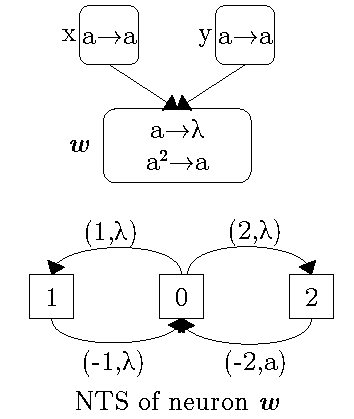
\includegraphics[scale=0.65]{fig-lts-1a.pdf}
      \caption{}
      \label{fig-nts-1a}
   \end{subfigure}
   \begin{subfigure}{.49\textwidth}
      \centering
      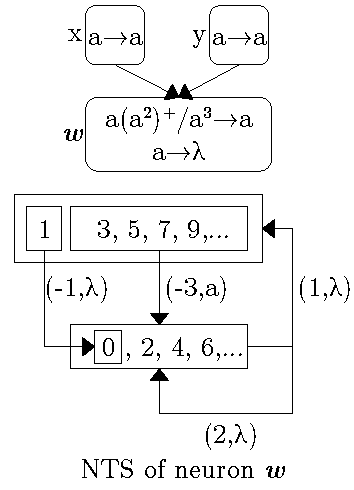
\includegraphics[scale=0.65]{fig-lts-1b.pdf}
      \caption{}
      \label{fig-nts-1b}
   \end{subfigure}
   \caption{Examples of Neurons and their NTSs}
   \label{fig-nts-1}
\end{figure}

%===================================================================================================

Figure \ref{fig-nts-2} highlights the effect of the behavior of the neuron subsystem to the neuron's
NTS. Figure \ref{fig-nts-2a}'s neuron $w$ and Figure \ref{fig-nts-2b}'s neuron $w$ have the same 
rule set with the single rule $a^3\ra a$ but have different subsystems. In Figure \ref{fig-nts-2a}, 
the subsystem (neurons $x,y,z$) sends a total of 3 spikes to neuron $w$ and the spikes are sent one 
spike at a time. In Figure \ref{fig-nts-2b}, the subsystem also sends a total of 3 spikes to neuron 
$w$ but there are four different ways for the $3$ spikes to arrive at neuron $w$. These four ways 
are: (1) $3$ spikes are sent one at a time, (2) $1$ spike is sent first then $2$ spikes are sent 
later, (3) $2$ spikes sent first then $1$ spike is sent later, and (4) $3$ spikes are sent at the 
same time. Different behavior of the subsystems imply different sets of transitions and hence 
different NTSs.

%===================================================================================================

\begin{figure}[H]
   \centering
   \begin{subfigure}{0.49\textwidth}
      \centering
      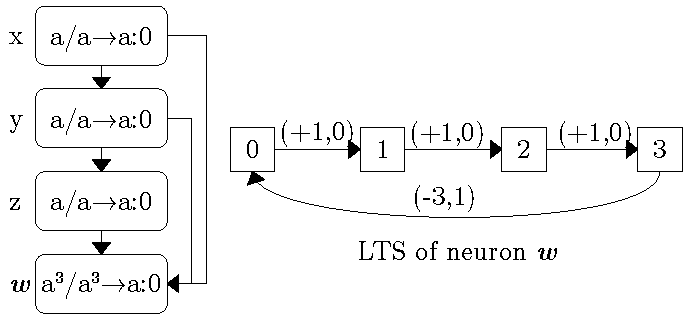
\includegraphics[scale=0.60]{fig-lts-2a.pdf}
      \caption{}
      \label{fig-nts-2a}
   \end{subfigure}
   \begin{subfigure}{0.49\textwidth}
      \centering
      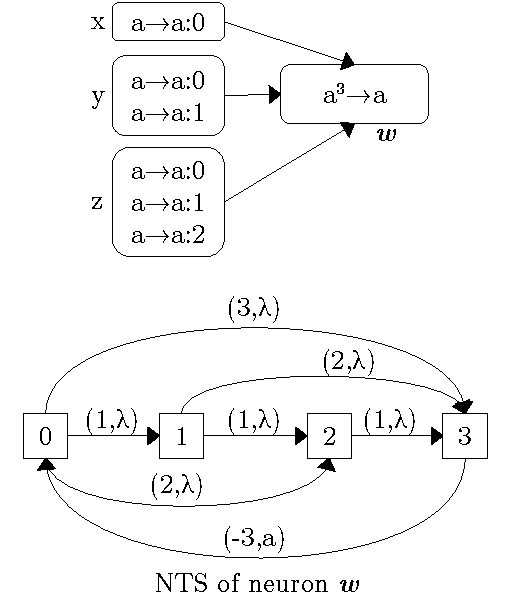
\includegraphics[scale=0.60]{fig-lts-2b.pdf}
      \caption{}
      \label{fig-nts-2b}
   \end{subfigure}
   \caption{Neurons with same rule set but different NTSs}
   \label{fig-nts-2}
\end{figure}

%===================================================================================================
\subsection{Operations on Neuron Transition Systems}\label{sec-homo-ops}
%===================================================================================================

\comment
{
We will define two operations on labelled transition systems, \emph{LTS translation} and \emph{LTS
scaling}. The idea behind these operations is that they take an LTS and a parameter $\delta$ and 
produce a new LTS that behaves exactly like the original LTS. When you are combining two different
rule sets from two different neurons in order to have common rule set, simply getting the union of
the two rule sets can cause conflicts. For example, let $\{a \ra a, a^2/a\ra a\}$ be the rule set 
of neuron $x$ and $\{a\ra\lambda,a^2/a\ra a\}$ be the rule set of neuron $y$. If we simply combine
the rule sets to have the common rule set $\{a\ra\lambda,a\ra a, a^2/a\ra a\}$ for both neurons
$x$ and $y$, there will be an unwanted behavior. If neuron $x$ has $1$ spike it
should use the rule $a\ra a$ and if neuron $y$ has $1$ spike it should use the rule $a\ra \lambda$.
If neurons $x$ and $y$ use the common rule set, when they have $1$ spike both of them will have
a non-deterministic choice, use rule $a\ra \lambda$ or use rule $a\ra a$. This non-determinism is 
an unwanted behavior that is the result of rule $a\ra\lambda$ `conflicting' with rule $a\ra a$. The 
common rule set changes the behavior of both neuron $x$ and neuron $y$. LTS translation and LTS 
scaling will be used to avoid such conflicts and changes in the neurons' behavior when combining
different rule sets. 
}

%===================================================================================================

\begin{definition2}[NTS Translation]
\emph{NTS translation} is an operation on an entire NTS. It takes a neuron transition system $nts=
(S,V,\ra)$ and a natural number $\delta$ and produce the neuron transition system $nts'=(S',V,\ra')$
where:
\begin{itemize}
   \item $S'=\{s+\delta\se|\se s \in S\}$. $s+\delta = \{i+\delta\se|\se i\in s\}$. We say that $s+
         \delta$ is \emph{state $s$ translated by $\delta$}.
   \item $\ra'=\{t+\delta \se|\se t\in \ra \}$. If $t=(s, (\alpha,\beta))$, $t+\delta=(s+\delta,
         (\alpha,\beta))$. We say that $t+\delta$ is \emph{transition $t$ translated by $\delta$}. 
         The translation of a transition $t$ by $\delta$ is simply the translation of the state
         component $s$ by $\delta$.
\end{itemize}
We denote $nts'$ as $nts+\delta$. We say that $nts+\delta$ is the neuron transition system $nts$
\emph{translated by $\delta$}.
\end{definition2}

%===================================================================================================

When you translate an NTS of some neuron $w$, the resulting new NTS is a neuron transition system 
of a different neuron, say neuron $w'$. For neurons, we will use an operation called \emph{neuron
translation}. Neuron translation is the analogue of NTS translation. NTS translation operates on
NTSs while neuron translation operates on neurons.

%===================================================================================================

\begin{definition2}[Neuron Translation]
\emph{Neuron translation} is an operation on a neuron. It takes a neuron $\sigma=(n,R)$ and a
natural number $\delta$ and produce the neuron $\sigma'=(n+\delta, R')$ where 
$R'=\{a^{\delta}E/a^c \ra \beta\se|\se E/a^c\ra \beta \in R\}$.
\end{definition2}

%===================================================================================================

A $\delta$-translation of neuron $w$ involves adding $\delta$ spikes to the neuron's initial spike
count and \emph{$\delta$-translating} the rules of the neuron. $\delta$-translating a rule 
$E/a^c\ra \beta$ means changing the regular expression of the rule to $a^{\delta}E$ 
($\delta$-translation of regular expression $E$). 

Figure \ref{fig-nts-3} shows neuron $w'$ which is a $\delta$-translated version of neuron $w$
from Figure \ref{fig-nts-1a} and the NTS of neuron $w'$ which is a $\delta$-translated version of
the NTS of neuron $w$. Neuron $w$ has $0$ initial spikes and the rules $a\ra\lambda$ and $a^2\ra a$. 
Neuron $w'$, being a $\delta$-translated neuron $w$, has $\delta$ initial spikes and has rules
$a^{\delta+1}/a\ra\lambda$ and $a^{\delta+2}/a\ra a$. The rules of neuron $w'$ are 
$\delta$-translated rules of neuron $w$. The translated rules in neuron $w'$ have the same actions
and consume the same amount of spikes and only the regular expressions are modified 
($\delta$-translated). The NTS of neuron $w'$, being a $\delta$-translated NTS of neuron $w$, has
all $\delta$-translated transistions of the NTS of neuron $w$. 

%===================================================================================================

\begin{figure}[H]
   \centering
   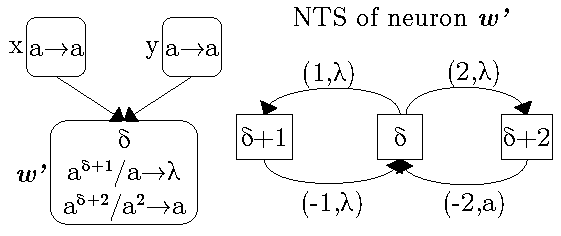
\includegraphics[scale=0.70]{fig-lts-3.pdf}
   \caption{Neuron $w'$ and its NTS}
   \label{fig-nts-3}
\end{figure}

%===================================================================================================

\begin{lemma}
A neuron and a translated version of the neuron have the same behavior.
\end{lemma}

\begin{proof}
Let neuron $w'$ with LTS $lts'$ be a $\delta$-translated version of some neuron $w$ with LTS $lts$. 
If neuron $w$ has an initial $n_0$ spikes, then neuron $w'$ has an initial $n_0+\delta$ spikes. Let 
$T_0$ be the set of transition in $lts$ such that $(s,(\alpha,\beta))\in T_0$ if and only if 
$n_0\in s$. Let $T'_0$ be the corresponding set for $lts'$. i.e. $T_0'=\{(s',(\alpha',\beta'))\se|\se
n_0+\delta \in s'\}$. If $(s,(\alpha,\beta))\in T_0$, then $(s+\delta,(\alpha,\beta)) \in T'_0$ since
$n_0\in s$ and $n\in s$ implies $n_0+\delta \in s+\delta$. If  $(s+\delta,(\alpha,\beta)) \in T'_0$,
then $(s,(\alpha,\beta))\in T_0$ since $n_0+\delta \in s+\delta$ and $n_0+\delta \in s+\delta$ implies
$n_0\in s$ (by reversing the $\delta$-translation of state $s+\delta$). This means that the 
transitions in $T'_0$ are all $\delta$-translated transitions of $T_0$. Since transition translation
does not change the label $(\alpha,\beta)$, the transitions in $T_0$ has the same set of labels as
the transitions in $T'_0$. This means that neuron $w$ at $n_0$ spike count and neuron $w'$ at $n_0+
\delta$ have the same set of actions they can perform. The same argument can be used for when neuron
$w$ has spike count $n$ (which is not necessarily the initial spike count) while neuron $w'$ has
spike count $n+\delta$.
\end{proof}

%===================================================================================================

\begin{definition2}[NTS Scaling]
\emph{NTS scaling} is an operation on an entire NTS. It takes a neuron transition system $nts=
(S,V,\ra)$ and a natural number $\delta$ and produce the neuron transition system $nts'=(S',V',\ra')$
where:
\begin{itemize}
   \item $S'=\{\delta s\se|\se s \in S\}$. $\delta s = \{\delta i\se|\se i\in s\}$.
         We say that $\delta s$ is \emph{state $s$ scaled by $\delta$}.
   \item $V'=\{(\delta \alpha,\beta)\se|\se (\alpha,\beta)\in V\}$.
   \item $\ra'=\{\delta t \se|\se t\in \ra \}$. If $t=(s, (\alpha,\beta))$, $\delta t=(\delta s,
         (\delta \alpha,\beta))$. We say that $\delta t$ is \emph{transition $t$ scaled by 
         $\delta$}. The scaling transition $t$ by $\delta$ means scaling its state component $s$ and
         $\alpha$ component by $\delta$.
\end{itemize}
We denote $nts'$ as $\delta\cdot nts$. We say that $\delta\cdot nts$ is the neuron transition system 
$nts$ \emph{scaled by $\delta$}.
\end{definition2}

%===================================================================================================

When you scale an NTS of some neuron $w$, the resulting new NTS is a neuron transition system 
of a different subsystem, say neuron $w'$ subsystem . If neuron translation is the analogue of NTS 
translation, \emph{subsystem scaling} is the analogue of NTS scaling. NTS scaling operates on NTSs 
while subsystem scaling operates on neuron subsystems.

%===================================================================================================

\begin{definition2}[Subsystem Scaling]
\emph{Subsystem scaling} is an operation on an SNP subsystem. Let neuron $\sigma=(n,R)$ and the all 
neurons $x$ connected to neuron $\sigma$ be collectively known as subsystem $sub$. \emph{Type 1 
subsystem scaling} takes a subsystem $sub$ and a natural number $\delta$ and produces a new 
subsystem $sub'$ where:
\begin{itemize}
   \item $sub'$ contains neuron $\sigma'=(\delta n, R')$. $R'=\{\delta E/a^{\delta c} \ra \beta\se|
         \se E/a^c\ra \beta \in R\}$. $\delta E$ is the regular expression that is the result of 
         replacing all instances of subexpression $a$ in $E$ by the subexpression $a^{\delta}$. i.e.
         If $E=a(a^2)^*$, then $\delta E = a^{\delta}((a^{\delta})^2)^* = a^{\delta}(a^{2\delta})^*$.
         We call this regular expression operation as \emph{regular expression scaling}. \emph{Rule
         scaling} is the operation where you scale the rule's regular expression and scale the
         number of spikes the rule consumes by the same amount $\delta$.
   \item if neuron $x$ is connected to neuron $\sigma$, then $\delta$ copies of neuron $x$ are
         connected to neuron $\sigma'$ and all these $\delta$ copies of neuron $x$ are also in 
         subsystem $sub'$. 
\end{itemize}

In \emph{Type 2} subsystem scaling, $sub'$ also contains the same neuron $\sigma'=(\delta n,R')$ 
described above. If in subsystem $sub$, neuron $x$ is connected to neuron $\sigma$, then neuron $x$
will also be in subsystem $sub'$ and for each neuron $x$ there will be additional $\delta$ neurons
called $x_1,..., x_{\delta}$ that have the same rule set with rules of the form $a^j\ra a^j$ where
$j$ is a number of spikes a rule in neuron $x$ can produce. Instead of  neuron $x$ being connected 
to neuron $\sigma'$, neuron $x$ will be connected to neurons $x_1,...,x_{\delta}$ while neurons 
$x_1,...,x_{\delta}$ will be connected to neuron $\sigma'$.
\end{definition2}

%===================================================================================================

Figure \ref{fig-nts-4} shows an NTS which is a $\delta$-scaling of the NTS of neuron $w$ from 
Figure \ref{fig-nts-1b}. The NTS of neuron $w$ from Figure \ref{fig-nts-1b} has the following 
transitions: $(\{1\}, (-1,\lambda))$, $(\{2i+1\}_{i\geq 1},(-3,a))$,$(\{2i\}_{i\geq 0},(1,\lambda))$, 
$(\{2i\}_{i\geq 0},(2,\lambda))$. The NTS in Figure \ref{fig-nts-4} has the following transitions:
$(\{\delta\}, (-\delta,\lambda))$, $(\{2i\delta+\delta\}_{i\geq 1},(-3\delta,a))$,
$(\{2i\delta\}_{i\geq 0},(\delta,\lambda))$, $(\{2i\delta\}_{i\geq 0},(2\delta,\lambda))$. All 
transitions in the NTS in Figure \ref{fig-nts-4} are all $\delta$-scaled versions of transitions in
the NTS in Figure \ref{fig-nts-1b}.

Figure \ref{fig-nts-4a} shows neuron $w'$ subsystem which that is the result of a type 1 subsystem 
$\delta$-scaling of the neuron $w$ subsystem in Figure \ref{fig-nts-1b}.

%===================================================================================================

\begin{figure}[H]
   \centering
   \begin{subfigure}{.49\textwidth}
      \centering
      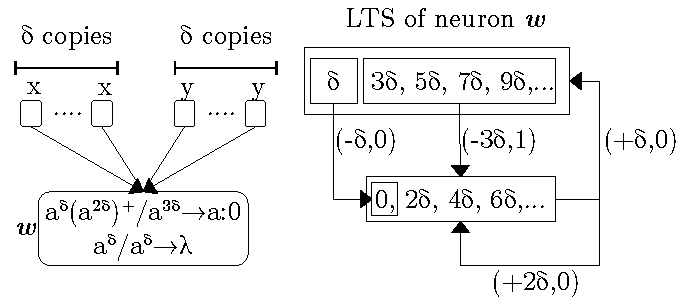
\includegraphics[scale=0.65]{fig-lts-4a.pdf}
      \caption{Type 1 Subsystem Scaling}
      \label{fig-nts-4a}
   \end{subfigure}
   \begin{subfigure}{.49\textwidth}
      \centering
      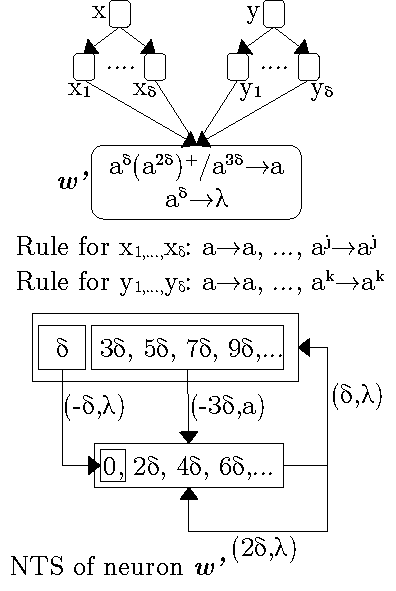
\includegraphics[scale=0.65]{fig-lts-4b.pdf}
      \caption{Type 2 Subsystem Scaling}
      \label{fig-nts-4b}
   \end{subfigure}
   \caption{NTS Scaling and Subsystem Scaling}
   \label{fig-nts-4}
\end{figure}

%===================================================================================================
\subsection{Procedures for Homogenizing Neurons' Rule Sets}\label{sec-homo-algo}
%===================================================================================================

SECTION INTRO PARAGRAPH

\begin{definition2}[Rule Transitions]
A rule set $R$ is a set of rules $\{r_1,...,r_i,...,r_n\}$ where each rule $r_i$ has the form 
$(s_i,a_i)$. For rule $r_i=(s_i,a_i)$, $s_i$ is called the state while $a_i$ is called action.
The \emph{scope} of a rule set $R=\{(s_1,a_1),...,(s_n,a_n)\}$, denoted by $scope(R)$, is the state 
$s = s_1 \cup s_2 \cup \cdots \cup s_n$.
\end{definition2}

SHORT INFO ON RULE SET, why rule set

\begin{definition2}[State-Actions Pair]
Given a rule set $R=\{(s_1,a_1),...,(s_n,a_n)\}$, we can associate a set of actions to any spike 
count $c$ in the scope of the rule set $R$. Let spike count $c$ be in the scope of $R$, $c\in 
scope(R)$, the actions associated with spike count $c$, denoted by $act(c)$, is the set 
$\{a_i\se |\se (s_i,a_i) \in R, c\in s_i\}$. We say that ``$act(c)$ is the set of actions at spike
count $c$". A set of actions can also be associated with a set of spike counts instead of simply
being associated with a single count. We say that set of spike counts $C$ is associated with actions
$act(C)$ if for all $c \in C$ the actions $act(c)$ at spike count $c$ is equal to $act(C)$. i.e. All
spike counts in $C$ have the same set of actions.
spike count,
\end{definition2}

MOTIVATION EXAMPLES

\begin{definition2}[Partition-Actions Set]
DEF
\end{definition2}


For example, $R = \{(s_1,a_1),(s_2,a_2),(s_3,a_3)\}$
$A = s_1\backslash (s_2 \cap s_3)$ 
$B = s_2\backslash (s_1 \cap s_3)$ 
$C = s_3\backslash (s_1 \cap s_2)$ 
$D = (s_1 \cup s_2 ) \backslash s_3$ 
$E = (s_1 \cup s_3 ) \backslash s_2$ 
$F = (s_2 \cup s_3 ) \backslash s_1$ 
$G = (s_1 \cup s_2 \cup s_3 )$ 

\begin{figure}[H]
    \centering
    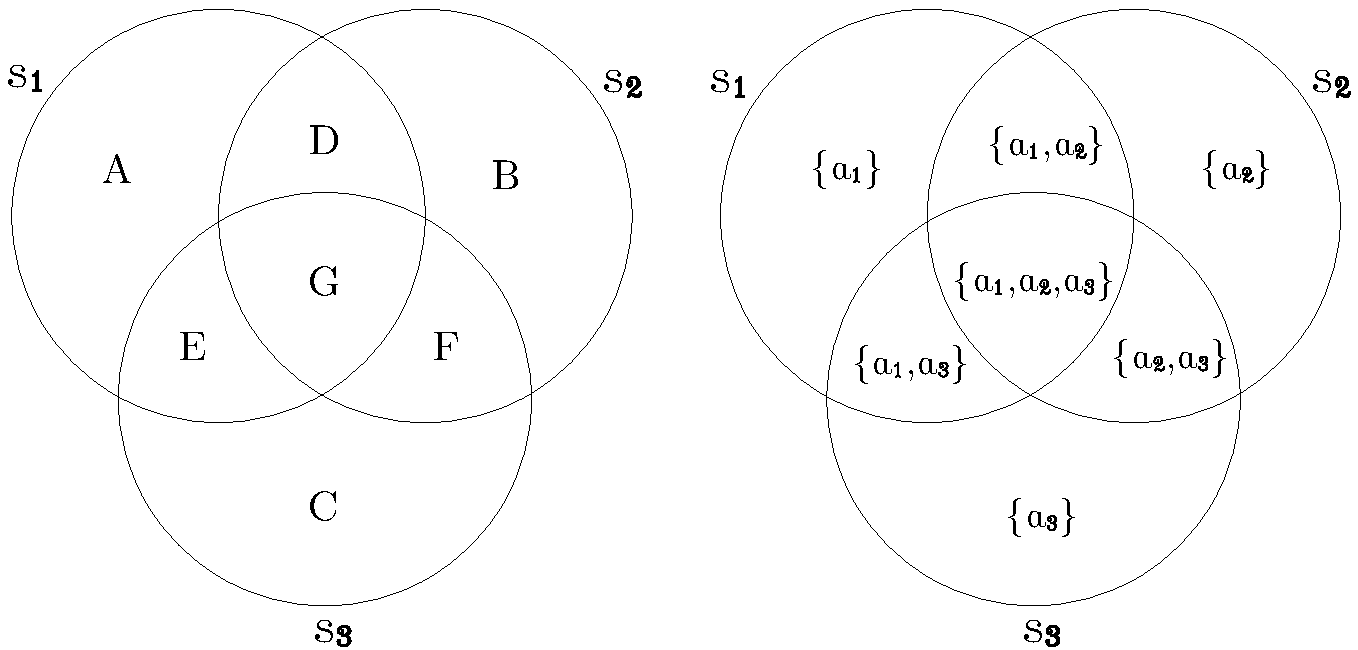
\includegraphics[scale=0.35]{fig-partitions-1.pdf}
    \caption{Partitions and Actions}
    \label{fig-partition-1}
\end{figure}

ELABORATE AND GIVE EXAMPLES(3)
%===================================================================================================

\begin{algorithm}[H]
\SetAlgoLined
\SetKwInput{KwInput}{Input}
\SetKwInput{KwOutput}{Output}
\KwInput{$R = \{(s_1,a_1),...,(s_n,a_n)\}$}
\KwOutput{$P = \{(p_1,A_1),...,(p_m,A_m)\}$}
$P \leftarrow \{\}$\;
\For{each $T \subseteq R$}
{
   $S   \leftarrow \{s_k \se|\se (s_k,a_k) \in T\}$             \;
   $S'  \leftarrow \{s_l \se|\se (s_l,a_l) \in R\backslash T\}$ \;
   $A_i \leftarrow \{a_k \se|\se (s_k,a_k) \in T\}$             \; 
   $p_i \leftarrow \Big(\bigcap\limits_{s_k \in  S} s_k \Big)  
                   \Big\backslash 
                   \Big(\bigcup\limits_{s_l \in S'} s_l \Big)$   \;
   \If{$p_i \neq \varnothing$}
   {
      Add $(p_i, A_i)$ to $P$ \;
   }
}

\For{each $(p_x,A_x),(p_y,A_y) \subseteq P$}
{
   \If{$A_x = A_y$}
   {
      Remove $(p_x,A_x)$ and $(p_y,A_y)$ from $P$\;
      Add $(p_x \cup p_y, A_x)$ to $P$ \;
   }
}
\caption{$GetPartitionActionsSet(R):$ \\Get the Partition-Actions Set that corresponds to rule
        transition set $R$}
\end{algorithm}

%===================================================================================================

\begin{definition2}[Compatibility of Two Partition-Actions Sets] Two partition-actions sets, 
$P=\{(p_i,A_i)\}$ and $P'=\{(p'_j,A'_j)\}$, are compatible if for all $c \in scope(P) \cup 
scope(P')$ there is a $(p_i, A_i)\in P$ and a $(p'_j,A'_j) \in P'$  such that $c\in p_i$,
$c\in p'_j$, and $A_i=A'_j$.
\end{definition2}
%===================================================================================================

\begin{algorithm}[H]
\SetAlgoLined
\SetKwInput{KwInput}{Input}
\SetKwInput{KwOutput}{Output}
\KwInput{$P = \{(p_1,A_1),...,(p_n,A_n)\}, P' = \{(p'_1,A'_1),...,(p'_m,A'_m)\}$}
\KwOutput{True or False}
$s  \leftarrow scope(P)$\;
$s' \leftarrow scope(P')$\;
$P  \leftarrow \{(p_1\cap s', A_1),...,(p_n\cap s', A_n)\}$\;
$P' \leftarrow \{(p'_1\cap s, A'_1),...,(p'_n\cap s, A'_m)\}$\;
\eIf{$P = P'$}
{
   return true;
}
{
   return false;
}
\caption{$Compatible(P,P')$\\
Return $true$ if partition-actions set $P$ is compatible with partition-actions set $P'$}
\end{algorithm}


%===================================================================================================
\begin{algorithm}[H]
\SetAlgoLined
\SetKwInput{KwInput}{Input}
\SetKwInput{KwOutput}{Output}
\KwInput{$\{R_1,...,R_p\}$}
\KwOutput{$R_0$}
$R_0 \leftarrow \{\}$\;
\For{each $R \in \{R_1,...,R_p\}$}
{
   $R_0 \leftarrow Merge(R_0,R)$\;
}
return $R_0$\;
\caption{Homogenization Algorithm}
\end{algorithm}

%===================================================================================================
\begin{algorithm}[H]
\SetAlgoLined
\SetKwInput{KwInput}{Input}
\SetKwInput{KwOutput}{Output}
\KwInput{$R_x,R_y$}
\KwOutput{$R_z$}
Convert rule set $R_x$ to partition-actions set $P_x$\;
Convert rule set $R_y$ to partition-actions set $P_y$\;
\eIf{$P_x$ is compatible with $P_x$}
{
   $R_Z \leftarrow R_x \cup R_y$\;
}
{
   Match $P_x$ and $P_y$\; 
   \For{each $(p_i,A_i) \in P_x$ and each $(p_j,A_j) \subseteq P_y$}
   {
   }
}
return $R_Z$\;
\caption{Merging Two Rule Sets}
\end{algorithm}


%===================================================================================================
\begin{algorithm}[H]
\SetAlgoLined
\SetKwInput{KwInput}{Input}
\SetKwInput{KwOutput}{Output}
\KwInput{$(p,A=(\alpha,\beta)),(p',A'=(\alpha',\beta'))$}
\KwOutput{(matching parameters)/no match}

\eIf{$\beta \neq \beta'$}
{
   return `no match'\;
}
{
   Solve $u_1\alpha+v_1=u_2\alpha'+v_2$\;
   //This linear diophantine equation is solved using Euclidean GCD algorithm\;
}
return $(u_1,v_1,u_2,v_2)$\;
\caption{Matching of Two Partition-Actions Pairs}
\end{algorithm}

%===================================================================================================
\section{Remarks and Conclusions}\label{sec-rem-con}
%===================================================================================================

\bibliographystyle{elsarticle-harv}
\bibliography{homogeneous-snp}

%===================================================================================================



 
\end{document}
